\documentclass[11pt]{article}

\usepackage[utf8]{inputenc}
\usepackage[T1]{fontenc}
\usepackage{lmodern}
\usepackage[margin=1in]{geometry}
\usepackage{microtype}
\usepackage{amsmath,amssymb}
\usepackage{booktabs}
\usepackage{multirow}
\usepackage{graphicx}
\usepackage{caption}
\usepackage{enumitem}
\usepackage{xurl}
\usepackage{xcolor}
\usepackage[colorlinks=true,linkcolor=blue,urlcolor=blue,citecolor=blue]{hyperref}
\usepackage[style=nature,backend=biber,maxbibnames=1,minbibnames=1,doi=false,url=false,isbn=false]{biblatex}
\addbibresource{references.bib}
\renewcommand*{\bibfont}{\small}
\setlength{\bibitemsep}{0pt}

\graphicspath{{figures/}{../figures/}}
\captionsetup{font=small,labelfont=bf}
\setlength{\parindent}{0pt}
\setlength{\parskip}{4pt}
\setlist[itemize]{leftmargin=*, itemsep=1pt, topsep=2pt}

\makeatletter
\renewcommand\section{\@startsection{section}{1}{\z@}%
    {-1.6ex \@plus -.5ex \@minus -.2ex}{0.7ex \@plus .2ex}%
    {\normalfont\large\bfseries}}
\renewcommand\subsection{\@startsection{subsection}{2}{\z@}%
    {-1.2ex \@plus -.4ex \@minus -.2ex}{0.4ex \@plus .2ex}%
    {\normalfont\normalsize\bfseries}}
\makeatother

% Red placeholders for anything that still needs final results. Delete before submitting:
% grep -n 'todo' final_report.tex should return only this definition.
\newcommand{\todo}[1]{\textcolor{red}{[TODO: #1]}}
% Include a figure if it exists (in figures/ or ../figures/), else draw a labelled placeholder,
% so the report compiles before every result is in.
\newcommand{\maybefig}[2]{\IfFileExists{figures/#2}{\includegraphics[#1]{#2}}{%
  \IfFileExists{../figures/#2}{\includegraphics[#1]{#2}}{%
  \fbox{\parbox[c][3cm]{0.8\textwidth}{\centering\vfill\todo{figure #2 not generated yet}\vfill}}}}}

\usepackage{titling}
\setlength{\droptitle}{-4em}
\title{\Large\bfseries Distilling Compact Gene Panels for Retinal Cell-Type Annotation\\
       Across Donors and Laboratories}
\author{Luana Liao (\href{mailto:ll3637@columbia.edu}{ll3637@columbia.edu}) \and
        Sky Sun (\href{mailto:ms6124@columbia.edu}{ms6124@columbia.edu})}
\date{December 2026}

\begin{document}
\maketitle
\vspace{-1.5em}

% ---------------------------------------------------------------------------
\begin{abstract}
\noindent
Targeted spatial transcriptomics measures only a few dozen to a few hundred genes, so the
gene panel must be chosen before the experiment. We asked how small a panel can identify
human retinal cell types in donors and labs it was not selected on. We trained a concrete
(Gumbel-softmax) gene selector, optionally with a donor-adversarial head, on the Human
Retina Cell Atlas (104 donors) and compared it with same-size panels of differentially
expressed (DE), highly variable and random genes, a 3{,}000-gene classifier, and
\todo{TranscriptFormer embeddings}. We evaluated on held-out donors, a held-out lab, and an
independent multiome dataset. Major cell classes were easy: a 25-gene DE panel reached
macro area under the precision--recall curve (auPR) 0.996 on held-out donors. The external
dataset and fine subtypes exposed real differences. \todo{One sentence on concrete vs DE
across k and tasks, with the paired-bootstrap result.} \todo{One sentence on the donor
adversary and the donor probe.} \todo{One sentence on ATAC support of learned vs DE panels.}
Code is available at \todo{GitHub URL}.
\end{abstract}

% ---------------------------------------------------------------------------
\section{Introduction}

Single-cell RNA sequencing measures thousands of genes per cell and is the standard way to
define cell types. Targeted spatial transcriptomics also records where each cell sits in the
tissue, but it detects only the genes for which probes were designed before the experiment.
Choosing this gene panel is a key design decision. The panel must be small, yet still tell
cell types apart in new samples from other donors and labs. The retina is a good test case.
Its cell types are well catalogued, from six major neuronal classes and glia down to more
than 100 subtypes, and large single-cell atlases now span many donors~\cite{li2026}.

We asked \emph{how small a gene panel can reliably identify human retinal cell types across
donors and labs}, and whether the selected genes make biological sense: do they match known
markers, and is their chromatin more accessible in the cell types they mark?

Gene panels are usually built from differential expression (DE): the top marker genes of
each cell type. Learned selectors instead choose genes jointly for a prediction task. The
concrete autoencoder~\cite{abid2019} makes feature selection differentiable with a
Gumbel-softmax relaxation~\cite{jang2017}, and PERSIST~\cite{covert2023} applies a similar
idea to spatial panel design. Pretrained single-cell models such as
TranscriptFormer~\cite{pearce2025} and Pan-human Azimuth~\cite{azimuth2026} offer another
route to annotation that needs no panel at all. \todo{One or two sentences on what these
prior works did not test that we do: cross-donor and cross-lab transfer, subtypes, and
chromatin support.}

Our contributions are:
\begin{itemize}
\item a benchmark of learned and DE-based gene panels of 10--200 genes on held-out donors,
a held-out lab and an independent dataset, for major classes and for bipolar (BC), retinal
ganglion (RGC) and amacrine (AC) subtypes;
\item a concrete selector with a class-conditional donor-adversarial head and a DE warm
start, and a direct test of how much donor information each panel carries;
\item a test of whether learned panels are better supported by cell-type-specific chromatin
accessibility than DE panels of the same size.
\end{itemize}

\begin{figure}[t]
\centering
\fbox{\parbox[c][4.2cm]{0.9\textwidth}{\centering\vfill
\todo{Figure 1: overview cartoon. HRCA (104 donors) $\rightarrow$ 3{,}000 HVGs $\rightarrow$
gene selector (DE / concrete / concrete + donor adversary) $\rightarrow$ $k$-gene panel
$\rightarrow$ same logistic regression $\rightarrow$ evaluate on held-out donors, held-out
lab, Wang 2022. Side branch: panel genes $\rightarrow$ Wang ATAC promoter accessibility.
Draw in PowerPoint/draw.io, export as PDF. The slide-3 diagram in the deck is a starting
point.}\vfill}}
\caption{\textbf{Overview.} \todo{caption}}
\label{fig:overview}
\end{figure}

% ---------------------------------------------------------------------------
\section{Methods}

\subsection{Data}

We downloaded both datasets as h5ad files from CZ CELLxGENE~\cite{cellxgene2025}. The HRCA
single-nucleus RNA sequencing (snRNA-seq) file holds 3{,}177{,}310 nuclei from 104 donors,
from six studies in two labs: Chen lab (Baylor, 87 donors) and Shekhar lab (Harvard, 17
donors). Fine subtype labels come from separate HRCA BC, AC and RGC files, joined on the
shared cell identifier. Wang et al.~\cite{wang2022} profiled 51{,}645 nuclei from 4 donors
with paired RNA and assay for transposase-accessible chromatin (ATAC-seq). Their file stores
only $\log(1+\mathrm{CP10k})$ values (counts per 10{,}000), so we recovered integer counts
by inverting the transform and dividing each cell by its smallest nonzero value. For ATAC we
used the authors' per-cell-type fragment files (13 cell types, GEO GSE196235).

We mapped Cell Ontology labels to 9 major classes shared by both datasets: rod, cone, BC,
AC, horizontal cell (HC), RGC, M\"uller glia (MG), astrocyte and microglia. For quality
control (QC), we kept cells with at least 300 detected genes and at most 10\% mitochondrial
reads, and removed doublets with Scrublet~\cite{wolock2019} per donor. We kept the 35{,}449
Ensembl genes shared by both datasets. The datasets share no donors. To balance classes, we
capped the major task at 400 cells per (donor, class) and the subtype tasks at 60 cells per
(donor, subtype), keeping subtypes with at least 300 atlas cells. This left 272{,}687 cells
for the major task and 68{,}700, 20{,}080 and 185{,}778 cells for 14 BC, 10 RGC and 71 AC
subtypes (Appendix Table~\ref{tab:data}).

\subsection{Evaluation}

All methods shared the same 5-fold donor-grouped stratified cross-validation, so each
donor's cells fell in exactly one test fold. Everything data-dependent (highly variable
genes (HVGs), z-score parameters, DE rankings, learned panels) was fit on training donors
only. Inputs were $\log(1+\mathrm{CP10k})$ of 3{,}000 seurat-v3 HVGs~\cite{stuart2019},
z-scored and clipped at $\pm10$. We also trained on Chen-lab donors and tested on the 17
Shekhar-lab donors (lab split), and applied each major-task model to Wang without retraining.
Every panel was scored with the same L2 multinomial logistic regression (LR) on its $k$ genes,
so differences reflect the genes, not the classifier. The primary metric was macro
one-vs-rest auPR. Differences between methods were tested with a paired donor bootstrap
(1{,}000 resamples of donors, both methods scored on the same resample).

\subsection{Gene panels}

\textbf{Baselines.} (i) LR on all 3{,}000 HVGs. (ii) Panels of $k\in\{10,25,50,100,200\}$
genes from the same HVGs: \emph{random} (3 seeds); \emph{HVG}, the top $k$ by variance rank;
and \emph{DE}, from Wilcoxon one-vs-rest tests in scanpy~\cite{wolf2018}, taking each
class's top up-regulated genes round-robin until $k$ distinct genes are chosen.
\todo{PERSIST, if run.}

\textbf{Concrete selector.} The selector has $k$ rows, each a categorical distribution over
the $G$ genes with logits $\boldsymbol\ell_j$. During training the selected features are
$\mathbf{x}^\top\mathrm{softmax}((\boldsymbol\ell_j+\mathbf{g})/T)$, where $\mathbf{g}$ is
Gumbel noise, and feed a 2-layer multilayer perceptron (MLP) with 256 units. At evaluation
each row takes its argmax gene. A penalty on any gene's total selection mass above 1
discourages duplicates. Following~\cite{abid2019} exactly (one learning rate, $T$ annealed
from 10 to 0.01) collapsed to the majority class, because the logits could not sharpen before
the selection hardened. Three changes fixed this: a separate learning rate for the logits
($5\times10^{-2}$); starting at $T_0=2$ and finishing the anneal at 75\% of training; and
inverse-frequency class weights. We trained 3 seeds per setting for 30 epochs.

\textbf{DE warm start.} In the DE-initialized variant, row $j$'s logits start peaked on the
$j$-th gene of the DE panel (logit gap 20, about 90\% of the row's mass at $T_0$), so
training starts from the DE panel and moves away only if that helps.

\textbf{Donor adversary.} A donor classifier sees the selected genes and the true class, and
is connected through gradient reversal~\cite{ganin2016} with weight $\lambda$. Conditioning on
class means only donor signal beyond class composition is penalized. We swept
$\lambda\in\{0, 0.1, 0.3, 1, 3\}$ on the lab split.

\subsection{Post-hoc analyses}

\textbf{Donor probe.} The adversary's own accuracy is a poor measure of donor information,
since the selector is trained against it. For each frozen panel we instead trained a fresh
LR to predict the donor from the panel genes, within each cell class, on the held-out donors
of that fold (half of each donor's cells for training, half for testing). We report
$(\mathrm{bacc}-c)/(1-c)$, where bacc is balanced accuracy and $c$ the chance level, so 0
means no donor signal and 1 means donors are fully identifiable.

\textbf{Chromatin support.} For each panel gene we took its target class (highest mean RNA
expression in HRCA) and computed its promoter specificity: $\log_2$ accessibility within
$\pm2$\,kb of the transcription start site in the target class minus the mean over the other
classes, from Wang pseudobulk ATAC. Because nearly any marker passes this check, we compared
learned panels with the DE panel of the same size and fold (label-permutation test), and with
expression-matched random genes (each gene replaced by a random HVG of the same expression
decile).

\textbf{Marker overlap and consensus panels.} We measured precision@$k$ against a list of
canonical retinal markers \todo{cite marker source}. Because learned panels vary between
folds, we also built a consensus panel from the $k$ genes selected most often across folds
and seeds, and scored it on Wang.

% ---------------------------------------------------------------------------
\section{Results}

\subsection{Major classes are easy within the atlas but not across labs}

The full LR reached macro auPR 1.000 on held-out donors and on the held-out lab, and a 25-gene
DE panel already reached 0.996. On Wang the full model dropped to 0.967, and small panels
dropped more: DE scored 0.786, 0.901 and 0.943 at $k=10$, 25 and 50 (Fig.~\ref{fig:bench}a).
The loss was concentrated in rare glia. At $k=50$, Wang microglia reached 0.75 auPR with the
DE panel and 0.71 with the concrete panel (0.89 with all genes), while every neuronal class
stayed at or above 0.95. HVG panels at $k=50$ largely missed Wang cones (auPR 0.51), so picking
genes per class beat picking by variance. \todo{Update with final concrete curve and the
consensus panel's Wang score.}

\begin{figure}[t]
\centering
\maybefig{width=\textwidth}{final_bench.png}
\caption{\textbf{Panel size vs error.} $1-$macro auPR (log scale, lower is better) against
panel size, mean $\pm$ s.d.\ over 5 donor folds \todo{and 3 seeds}. \textbf{a}, major classes
on Wang 2022 without retraining. \textbf{b--d}, subtypes on held-out HRCA donors. Dashed: the
3{,}000-gene LR.}
\label{fig:bench}
\end{figure}

\subsection{Learned panels beat DE only on some subtype tasks}

At $k=50$, the learned selector matched DE on BC subtypes, beat it on AC subtypes (0.955 vs.\
0.944) and lost on RGC subtypes (0.905 vs.\ 0.954). For AC, round-robin DE allots fewer than
one gene to each of the 71 classes, while a learned panel can use genes that separate several
subtypes at once. RGC has the least training data (about 16k cells per fold) and is dominated
by midget cells. \todo{Report the paired differences at every $k$ (Fig.~\ref{fig:paired}),
whether the DE warm start closes the RGC gap, and the lab-split subtype results.}

\begin{figure}[t]
\centering
\maybefig{width=0.8\textwidth}{final_paired.png}
\caption{\textbf{Learned vs DE panels.} Difference in macro auPR (learned $-$ DE) with paired
donor-bootstrap 95\% confidence intervals, one marker per seed. \todo{finalize}}
\label{fig:paired}
\end{figure}

\subsection{Panels carry little donor information, and the adversary adds little}

\todo{Donor probe (Fig.~\ref{fig:donor}): how identifiable donors are from DE, HVG and
learned panels compared with all 3{,}000 HVGs. Then the $\lambda$ sweep on the lab split
(Appendix Fig.~\ref{fig:lambda}). Interim: with $\lambda=1$, performance was unchanged or
slightly lower, and the gain on Wang (0.946 vs.\ 0.944) was within fold-to-fold noise.}

\begin{figure}[t]
\centering
\maybefig{width=0.9\textwidth}{final_donor_probe.png}
\caption{\textbf{Donor information in each panel ($k=50$).} Normalized balanced accuracy of a
donor classifier trained on held-out donors, within cell class. 0 = chance. \todo{finalize}}
\label{fig:donor}
\end{figure}

\subsection{Selected genes and chromatin support}

Learned panels were less stable than DE panels. Across folds at $k=50$, DE panels were nearly
identical (mean pairwise Jaccard index 0.90), but concrete panels were not (0.44). In fold~0,
21 of the 50 concrete genes were also in the DE panel, including canonical markers such as
\emph{SAG} (photoreceptors), \emph{PTPRC} (microglia) and \emph{CRB1} (MG). The concrete panel
also picked \emph{GAD1} (GABAergic AC), which DE did not. \todo{Consensus panel, precision@$k$
against markers, and the ATAC comparison with DE panels (Fig.~\ref{fig:atac}).}

\begin{figure}[t]
\centering
\maybefig{width=0.8\textwidth}{final_atac.png}
\caption{\textbf{Chromatin support.} Mean promoter-accessibility specificity of panel genes
for their target class, one point per fold and seed. Dotted: expression-matched random genes.
\todo{finalize}}
\label{fig:atac}
\end{figure}

% ---------------------------------------------------------------------------
\section{Discussion}

\todo{Did things turn out as expected? Draft points: (1) major classes are nearly solved by
small DE panels, so the hard and useful problem is transfer across labs and fine subtypes.
(2) DE is a strong baseline, as the course feedback predicted. Learned selection helps most
when there are many classes per gene (AC), and needs enough data per class (RGC). (3) Donor
effects are small compared with cell identity, which explains why the adversary had little
to remove. (4) Many different gene sets work about equally well, so a consensus panel is more
useful than any single fold's panel.}

\todo{Limitations: Wang has only 4 donors and 231 microglia. One external lab. Panels drawn
from 3{,}000 HVGs. snRNA-seq is not spatial data: a real panel would also face probe
efficiency and segmentation errors.}

\todo{Next steps: validate a panel on real spatial data (e.g. retina MERFISH/Xenium), extend
the ATAC test to subtypes, and try selectors that favour stable panels.}

\todo{Code and data: GitHub URL; processed data on Google Drive.}

\printbibliography

% ---------------------------------------------------------------------------
\appendix
\section{Supplementary data and figures}

\begin{table}[h]
\centering\small
\caption{Datasets after QC. Medians are per cell. UMI: unique molecular identifier.}
\label{tab:data}
\begin{tabular}{lrrrrr}
\toprule
 & cells & donors & classes & median genes & median UMIs \\
\midrule
HRCA major-class task & 272{,}687 & 104 & 9 & \multirow{4}{*}{2{,}671} & \multirow{4}{*}{5{,}592} \\
HRCA BC subtypes & 68{,}700 & 104 & 14 & & \\
HRCA RGC subtypes & 20{,}080 & 101 & 10 & & \\
HRCA AC subtypes & 185{,}778 & 104 & 71 & & \\
Wang 2022 (external test) & 51{,}504 & 4 & 9 & 1{,}425 & 2{,}649 \\
\bottomrule
\end{tabular}
\end{table}

\begin{figure}[h]
\centering
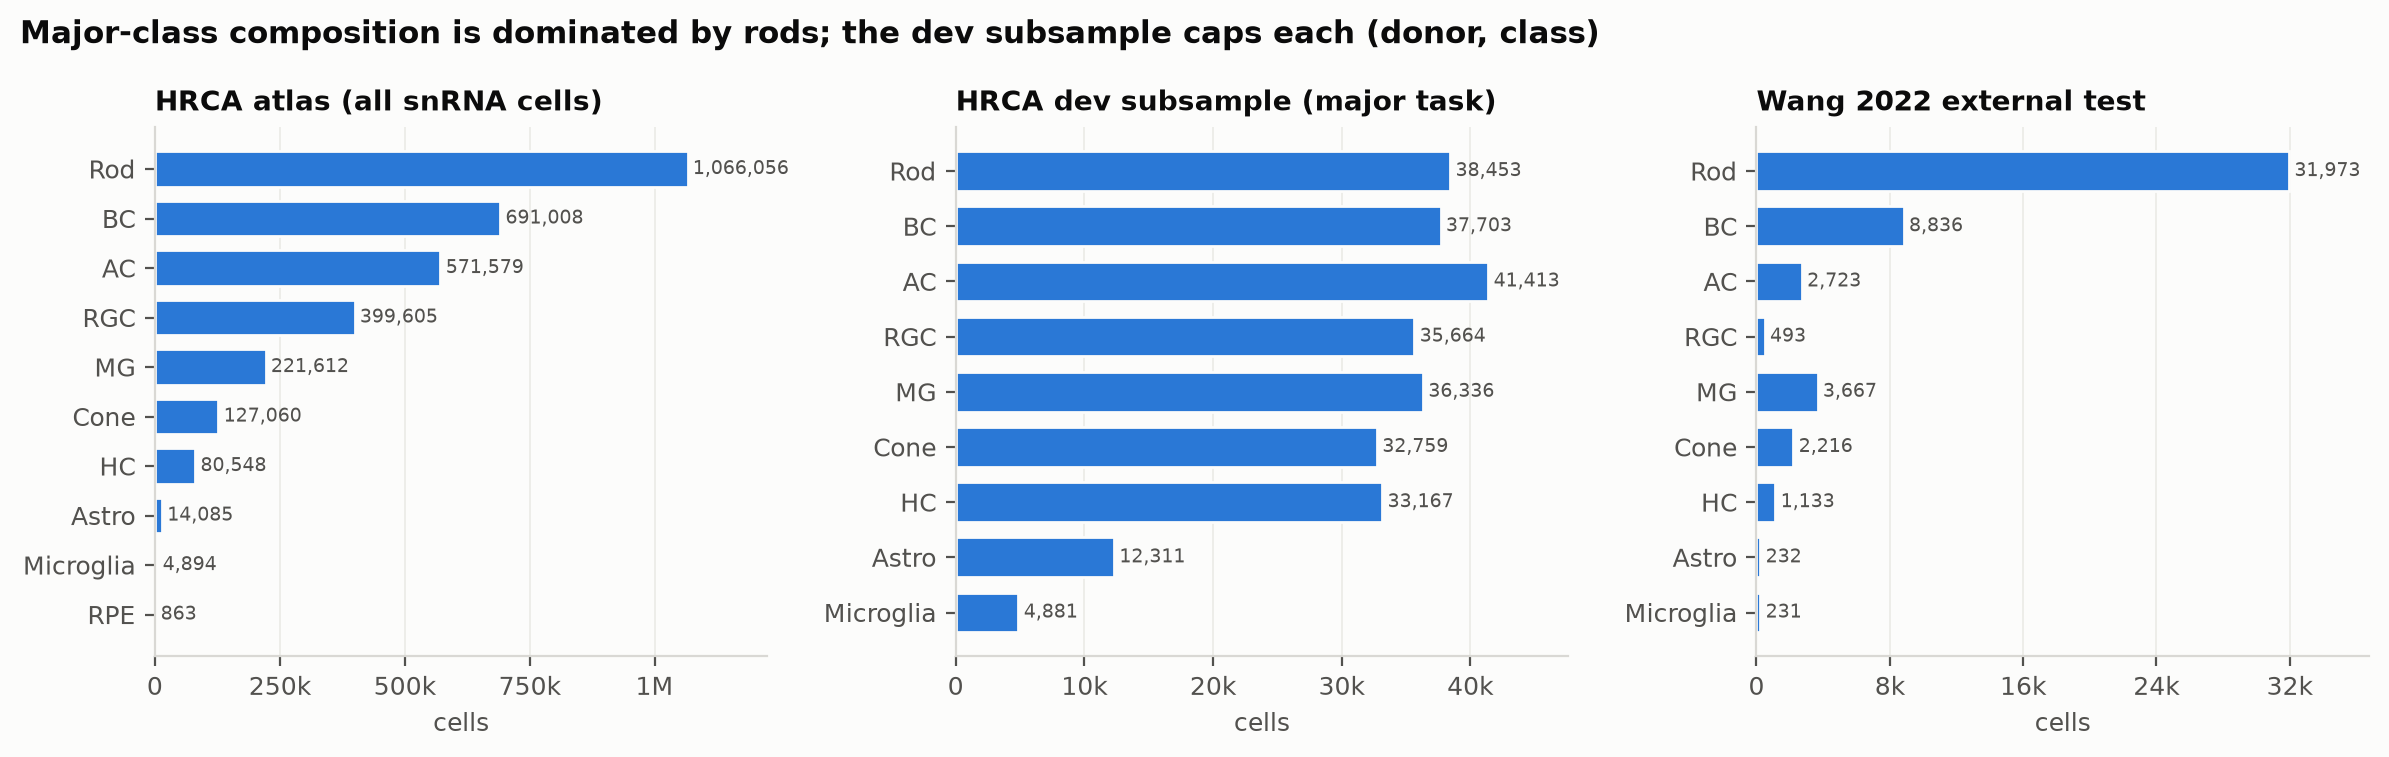
\includegraphics[width=0.8\textwidth]{eda_class_counts.png}
\caption{Major-class composition of the HRCA atlas, our development subsample and Wang 2022.}
\label{fig:counts}
\end{figure}

\begin{figure}[h]
\centering
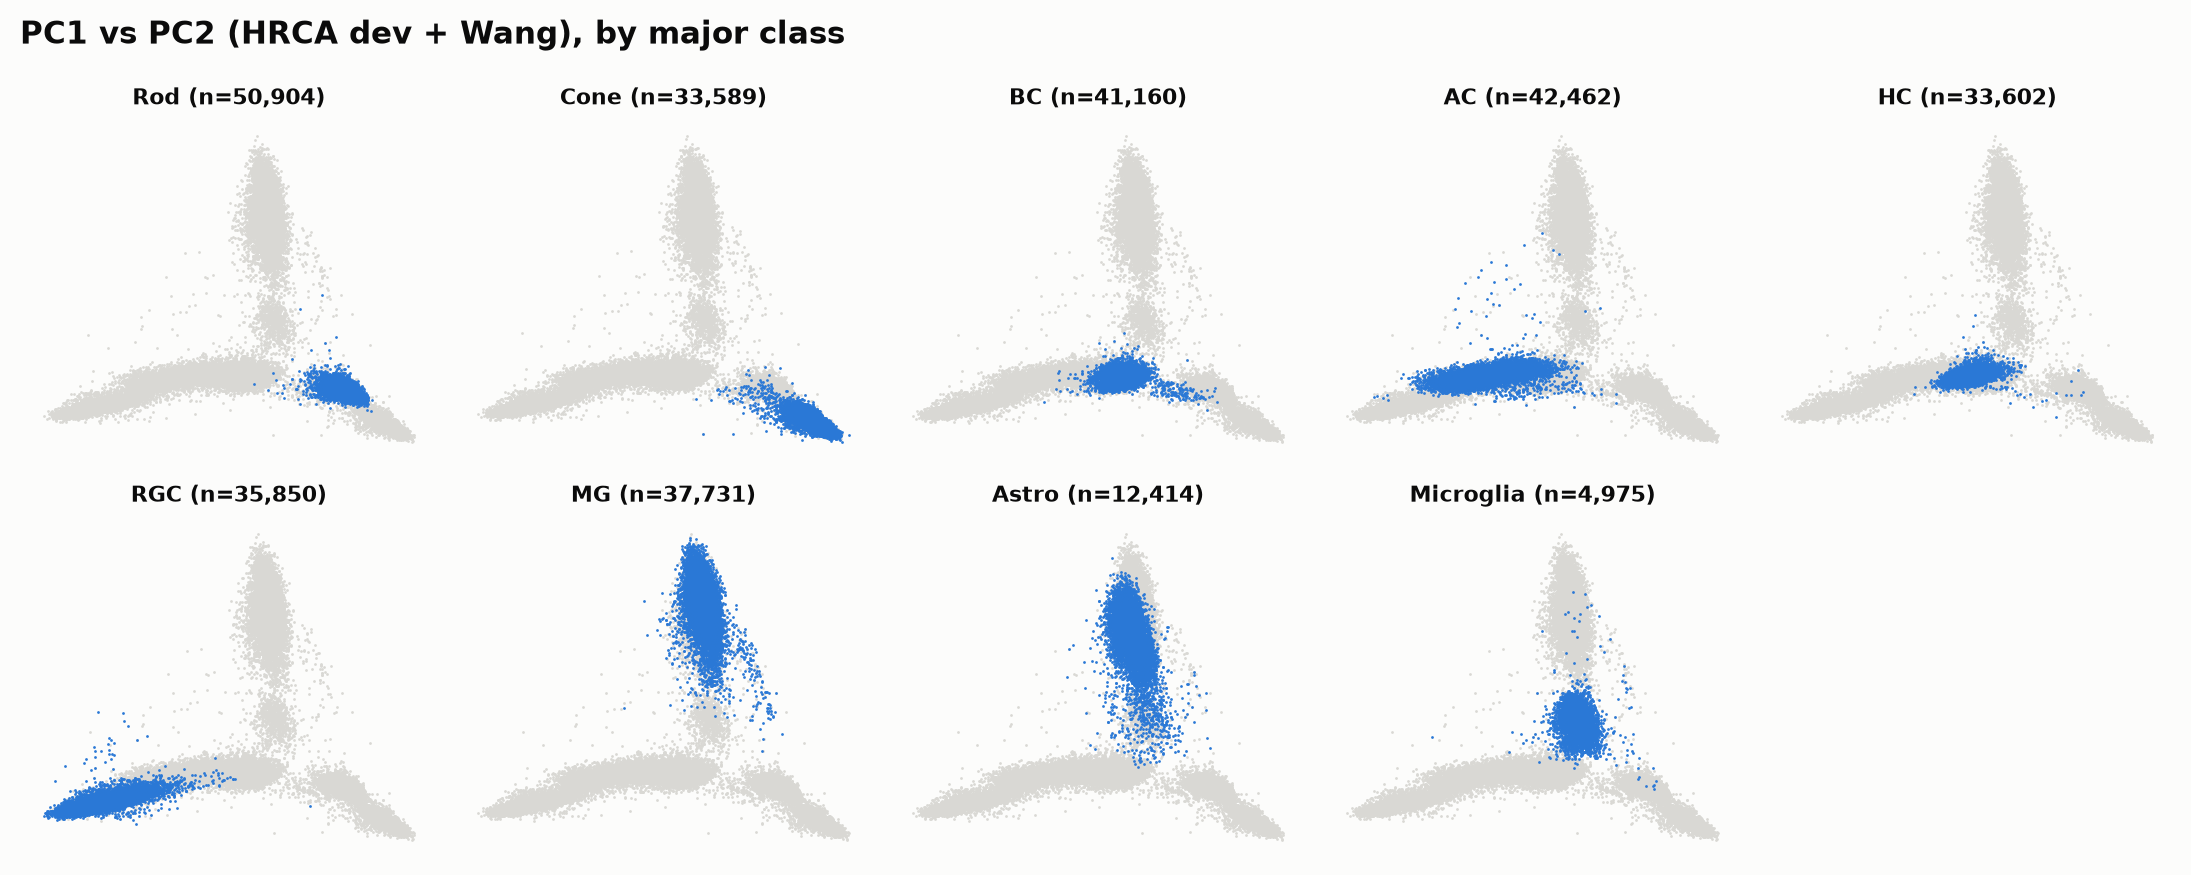
\includegraphics[width=0.85\textwidth]{eda_pca_by_class.png}\\[-1pt]
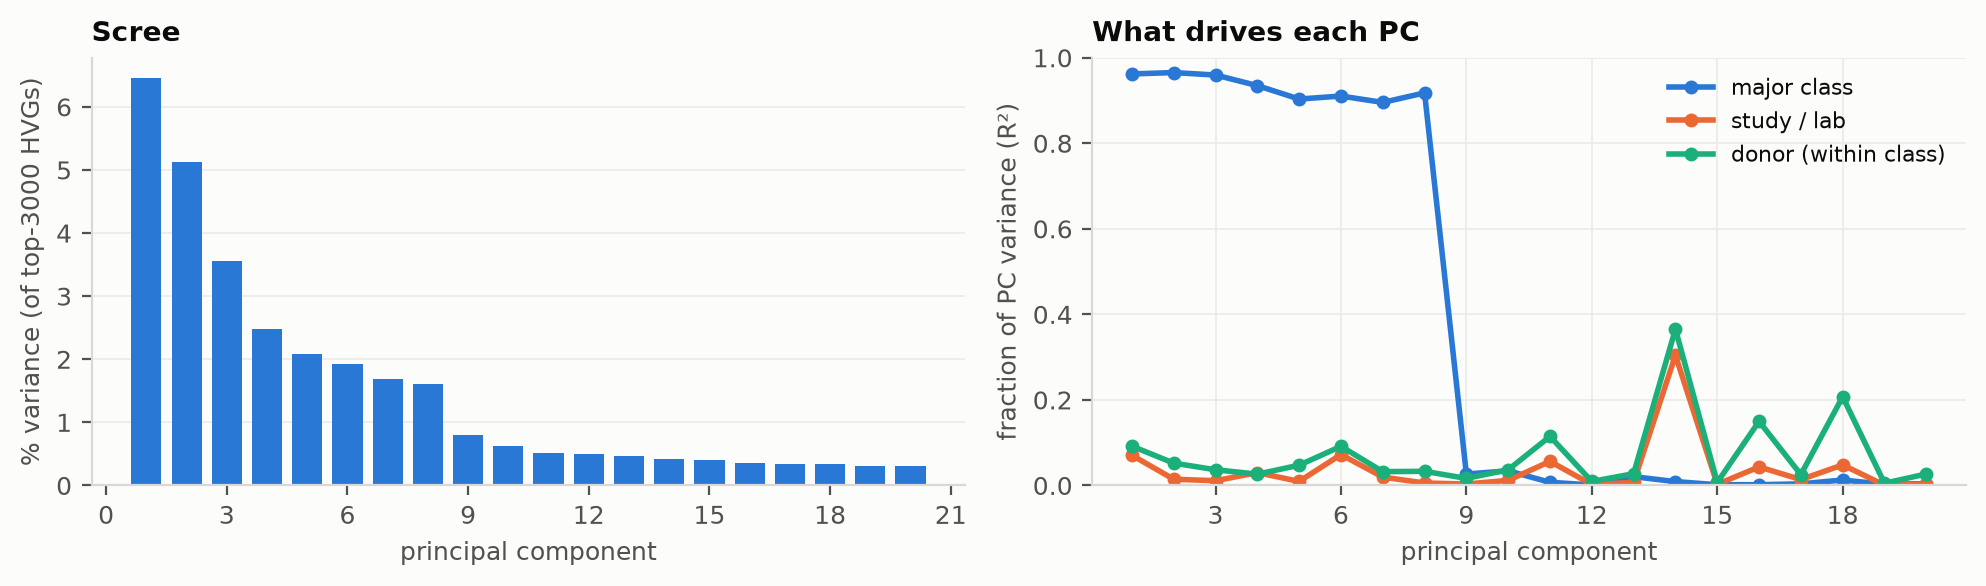
\includegraphics[width=0.72\textwidth]{eda_pca_variance.png}
\caption{\textbf{a}, PC1 vs.\ PC2 of HRCA major-task cells plus 20k Wang cells. \textbf{b},
fraction of each PC's variance explained by class, study/lab and donor within class. Class
explains 90--96\% of PCs 1--8 and donor less than 10\%.}
\label{fig:pca}
\end{figure}

\begin{figure}[h]
\centering
\maybefig{width=0.5\textwidth}{final_lambda.png}
\caption{Donor-adversarial weight $\lambda$ vs macro auPR at $k=50$. \todo{finalize}}
\label{fig:lambda}
\end{figure}

\end{document}
